% -----------------------------------------------------------------------------
% Trabalhos Relacionados
% -----------------------------------------------------------------------------

\chapter{Trabalhos Relacionados}
\label{chap:trabRelac}

Em 2012 \citeonline{BULENT} apresentaram um estudo sobre a qualidade do aprendizado na disciplina de Rede de Computadores no curso de graduação da universidade de Baskent. A analise foi feita no decorrer de três anos, de 2007 a 2010, e constatou que a utilização de ferramentas como simuladores e aplicativos, além de animações, melhoraram resultados obtidos pelos alunos. Foram feitas analises semanais sobre a performance dos estudantes no laboratório do curso e estas constataram que os alunos aprendem melhor quando envolvidos na aplicação pr\'atica da teoria do estudo de Redes de Computadores. Além disso questionários aplicados ao final de cada do curso constataram que os alunos estavam felizes em serem envolvidos na aplicação prática dos tópicos abordados pela disciplina durante as aulas de laboratório.


Um simulador com este objetivo, educacional, foi desenvolvido por \citeonline{POLETTI}, tendo como base um dos softwares citando anteriormente, o \textit{Cisco Packet Tracer}, em seu trabalho de conclusão de curso. O simulador desenvolvido por ele facilita a visualização das estruturas dos principais protocolos do modelo TCP/IP, sem a necessidade, que havia na ferramenta Cisco, de configurar uma rede virtual para poder simular o envio destes. Além disso a implementação permite interação direta do usuário com a estrutura dos protocolos, possibilitando mudanças da maioria dos valores de seus campos, e desta forma visualizar o impacto que tais mudanças causam na comunicação (o que era muito limitado na ferramenta original onde o conteúdo dos pacotes são estáticos). O novo simulador ainda possui o diferencial de ser uma ferramenta distribuída, o que permite a interação entre vários simuladores distintos.


Também com objetivo de ser didático \citeonline{LEE} desenvolveram um framework orientado à eventos chamado KENVSv2. Eles propõem a utilização deste à estudantes de Ciência da Computação, que devem implementar os drivers TCP e IP e protocolos de roteamento. A arquitetura proposta para o trabalho pode ser vista na Figura \ref{fig:KENVSv2}: o host virtual age como uma camada de aplicaç\~ao para o TCP e como link de dados combinados e camada física para o IP. Além de possuir um par em funcionamento para a realização de testes de comunicação. De acordo com seu artigo, eles acreditam que para o uma experi\^encia completa de aprendizado os alunos devem ser capaz de implementar e testar toda a pilha de protocolos.


\begin{figure}[H]
	\centering
    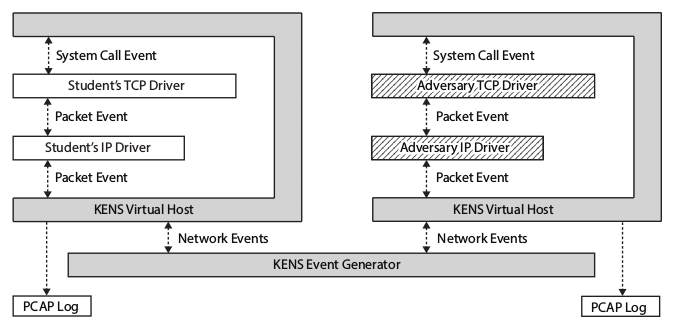
\includegraphics[width=0.85\textwidth]{04-figuras/KENVSv2.png}
    \caption{Funcionamento em camadas}
    \label{fig:KENVSv2}
    \fonte{\cite{LEE}}
\end{figure}  	 
	 